\documentclass[12pt]{article}

\usepackage{graphicx}			% Use this package to include images
\usepackage{amsmath}		
% A library of many standard math expressions
\graphicspath{ {./Images/} }
\usepackage[margin=1in]{geometry}% Sets 1in margins. 
\usepackage{fancyhdr}			% Creates headers and footers
\usepackage{enumerate}          %These two package give custom labels to a list
\usepackage[shortlabels]{enumitem}


% Creates the header and footer. You can adjust the look and feel of these here.
\pagestyle{fancy}
\fancyhead[l]{Aditya Gupta}
\fancyhead[c]{Math 134 Homework \#3}
\fancyhead[r]{\today}
\fancyfoot[c]{\thepage}
\renewcommand{\headrulewidth}{0.2pt} %Creates a horizontal line underneath the header
\setlength{\headheight}{15pt} %Sets enough space for the header



\begin{document} %The writing for your homework should all come after this. 


%Enumerate starts a list of problems so you can put each homework problem after each item. 
\begin{enumerate}[start=1,label={\bfseries. },leftmargin=1in] %You can change "Problem" to be whatevber label you like. 
    \item [\textbf{57.}]

    First, we find the slope of the tangent line:
    \[
    f'(3) = \lim_{h \to 0} \frac{(3 + h)^2 - 9}{h} = \lim_{h \to 0} \frac{6h + h^2}{h} = 6
    \]
    The equation of the tangent line is:
    \[
    y - 9 = 6(x - 3) \quad \Rightarrow \quad y = 6x - 9
    \]
    To find the x-intercept of the tangent line, set \( y = 0 \):
    \[
    0 = 6x - 9 \quad \Rightarrow \quad x = 1.5
    \]
    Thus, tangent intersects x axis at \( (1.5, 0) \).

    Next, the slope of the normal line is the negative reciprocal of the tangent line's slope, so it is \( -\frac{1}{6} \). Thus:
    \[
    y - 9 = -\frac{1}{6}(x - 3) \quad \Rightarrow \quad 6y-54 = 3-x
    \]
    To find the x-intercept of the normal line, set \( y = 0 \):
    \[
    0 = \frac{57-x}{6} \quad \Rightarrow \quad x = 57
    \]
    Thus, the normal line intersects the x-axis at \( (57, 0) \).

    Finally, the distance \( s \) between the x-intercepts is:
    \[
    s = 57 - 1.5 = 55.5
    \]
    Therefore, \( s = {55.5} \).

    \item [\textbf{59.}]
    
    \begin{enumerate}
        \item 
        To show that \( f(x) \) is continuous at \( x = 0 \), we check if:
        \[
        \lim_{x \to 0} f(x) = f(0).
        \]
        
        To calculate the limit, we use the squeeze theorem:
        \[
        -|x| < x\cdot sin\left(\frac{1}{x}\right) < |x|
        \]
        Since:
        \[
        \lim_{x\to0} -|x| = 0 \quad and \quad \lim_{x\to0}|x| = 0
        \]
        We obtain:
        \[
        \lim_{x\to0}x\cdot sin\left(\frac{1}{x}\right) = 0
        \]
        And since:
        \[
        f(0) = 0
        \]
        We conclude that $f(x)$ is continuous at 0
        \bigbreak
        To show $g(x)$ is continuous at 0,
        \[
        \lim_{x \to 0} g(x) = g(0).
        \]
        
        Using the squeeze theorem again:
        \[
         -x^2\leq x^2 \sin\left(\frac{1}{x}\right) \leq x^2,
        \]
        Since:
        \[
        \lim_{x \to 0} x^2 \sin\left(\frac{1}{x}\right) = 0 \quad and \quad \lim_{x \to 0} -x^2 \sin\left(\frac{1}{x}\right) = 0
        \]
        We obtain:
        \[
        \lim_{x\to0}g(x) = 0
        \]
        And since:
        \[
        g(0) = 0 \quad (\text{Since $g(0) = 0*f(0)$})
        \]
        We conclude that $g(x)$ is continuous at 0
        \bigbreak
    
    \item 
    
    To check the differentiability of \( f(x) \) at \( x = 0 \), we compute the derivative:
    \[
    f'(0) = \lim_{x \to 0} \frac{f(x) - f(0)}{x} = \lim_{x \to 0} \frac{x \sin\left(\frac{1}{x}\right)}{x}.
    \]
    This simplifies to:
    \[
    f'(0) = \lim_{x \to 0} \sin\left(\frac{1}{x}\right),
    \]
    which does not exist due to the oscillatory behavior of \( \sin\left(\frac{1}{x}\right) \). Thus, \( f(x) \) is not differentiable at 0.
    \bigbreak
    \item
    
    The derivative of \( g(x) \) at \( x = 0 \) is:
    \[
    g'(0) = \lim_{x \to 0} \frac{g(x) - g(0)}{x} = \lim_{x \to 0} \frac{x^2 \sin\left(\frac{1}{x}\right)}{x} = \lim_{x \to 0} x \sin\left(\frac{1}{x}\right).
    \]
    
   Since this is a prior result, we can say that $g'(0) = 0$ and $g(x)$ is differentiable at 0.
    
\end{enumerate}
\newpage
    \item [\textbf{50.}]
    To find A and B, we must obtain 2 equations about A and B such that we can solve them simultaneously and obtain a result.

    $f(x)$ = \begin{cases}
Ax^2 + B, &  x < -1\\
Bx^5 + Ax + 4, & x \geq -1
\end{cases}

We can equate the two parts of the piece-wise function for $x=-1$ since the function is everywhere continuous. We know this as in class it was shown that the everywhere continuity of the derivative implies that the original function is everywhere continuous.
\[
Ax^2 + B = Bx^5 + Ax + 4
\]
\[
Bx^5 - Ax^2 + Ax - B + 4 = 0
\]
Substituting in $x = -1$
\[
-B - A - A - B + 4 = 0
\]
\[
-2B - 2A + 4 = 0
\]
We will use the above result later:

Now differentiating $f(x)$

$f'(x)$ = \begin{cases}
    2Ax, & x<-1 \\
    5Bx^4 + A, & x\geq -1
\end{cases}

\[
2Ax = 5Bx^4 + A
\]
Substituting in $x=-1$
\[
-2A = 5B + A
\]
\[
A = \frac{-5B}{3}
\]
Substituting in the value of A in the original result

\[
-2B - 2\left(\frac{-5B}{3}\right) + 4 = 0
\]

\[
-2B + \frac{10B}{3} + 4 = 0
\]
\[
\frac{4B}{3} = -4
\]
\[
B = -3
\]

Since $A = \frac{-5B}{3}$, we find $A = 5$.
\boxed{A = 5, B = -3}

\item [\textbf{62.}]

    The derivative of \( f(x) = x^3 \) is:
    \[
    f'(x) = 3x^2
    \]
    At \( x = c \), the slope of the tangent line is:
    \[
    f'(c) = 3c^2
    \]
    The equation of the tangent line at \( x = c \) is given by the point-slope form:
    \[
    y - f(c) = f'(c)(x - c)
    \]
    Substituting \( f(c) = c^3 \) and \( f'(c) = 3c^2 \), we get:
    \[
    y - c^3 = 3c^2(x - c)
    \]
    Expanding this equation:
    \[
    y = 3c^2(x - c) + c^3 = 3c^2x - 3c^3 + c^3 = 3c^2x - 2c^3
    \]
    So the equation of the tangent line is:
    \[
    y = 3c^2x - 2c^3
    \]

    To find other solutions(should they exist), we will equate the tangent line to the function.

    \[
    x^3 = 3c^2x-2c^3
    \]
    \[
    x^3 -3c^2x + 2c^3 = 0
    \]
    Computing the roots for the equation, we obtain the following expansion:
    \[
    (x-c)(x^2+cx-2c^2)=0
    \]
    \[
    (x-c)(x-c)(x+2c) = 0
    \]
    Therefore, the tangent line intersects the function at $x=-2c$

    \item [\textbf{54.}]
    \begin{enumerate}
        \item The function \( g(x) \) is defined as \( g(x) = \begin{cases} x^3 & \text{for } x \geq 0 \\ 0 & \text{for } x < 0 \end{cases} \). To find \( g'(0) \), we use the limit definition of the derivative: 
\[
g'(0) = \lim_{h \to 0} \frac{g(h) - g(0)}{h} = \lim_{h \to 0} \frac{g(h)}{h}
\]
For \( h > 0 \), \( g(h) = h^3 \), so:
\[
g'(0) = \lim_{h \to 0^+} \frac{h^3}{h} = \lim_{h \to 0^+} h^2 = 0
\]
For \( h < 0 \), \( g(h) = 0 \), so:
\[
g'(0) = \lim_{h \to 0^-} \frac{0}{h} = 0
\]
Thus, \( g'(0) = 0 \). For the second derivative \( g''(0) \), we apply:
\[
g''(0) = \lim_{h \to 0} \frac{g'(h) - g'(0)}{h} = \lim_{h \to 0} \frac{g'(h)}{h}
\]
For \( h > 0 \), \( g'(h) = 3h^2 \), so:
\[
g''(0) = \lim_{h \to 0^+} \frac{3h^2}{h} = \lim_{h \to 0^+} 3h = 0
\]
For \( h < 0 \), \( g'(h) = 0 \), so:
\[
g''(0) = \lim_{h \to 0^-} \frac{0}{h} = 0
\]
Thus, \( g''(0) = 0 \).

        \item 

        \[
        g'(x) = \begin{cases}
            3x^2, & x\geq 0\\
            0, & x<0
        \end{cases}
        \]
        \[
        g''(x) = \begin{cases}
            6x, & x\geq 0\\
            0, & x<0
        \end{cases}
        \]

        \item To show that \( g'''(0) \) does not exist, we use the definition of the derivative:
\[
g'''(0) = \lim_{h \to 0} \frac{g''(h) - g''(0)}{h}
\]
Since \( g''(0) = 0 \), this simplifies to:
\[
g'''(0) = \lim_{h \to 0} \frac{g''(h)}{h}
\]
For \( h > 0 \), \( g(x) = x^3 \), so \( g'(x) = 3x^2 \) and \( g''(x) = 6x \), meaning \( g''(h) = 6h \) for \( h > 0 \). 

For \( h < 0 \), \( g(x) = 0 \), so \( g''(h) = 0 \). Now, evaluate the limit from both sides:
\[
g'''(0) = \lim_{h \to 0^+} \frac{6h}{h} = \lim_{h \to 0^+} 6 = 6
\]
\[
g'''(0) = \lim_{h \to 0^-} \frac{0}{h} = 0
\]
Since the left-hand and right-hand limits are not equal, \( g'''(0) \) does not exist due to a jump discontinuity.

\item 
\begin{figure}[h!]
    \centering
    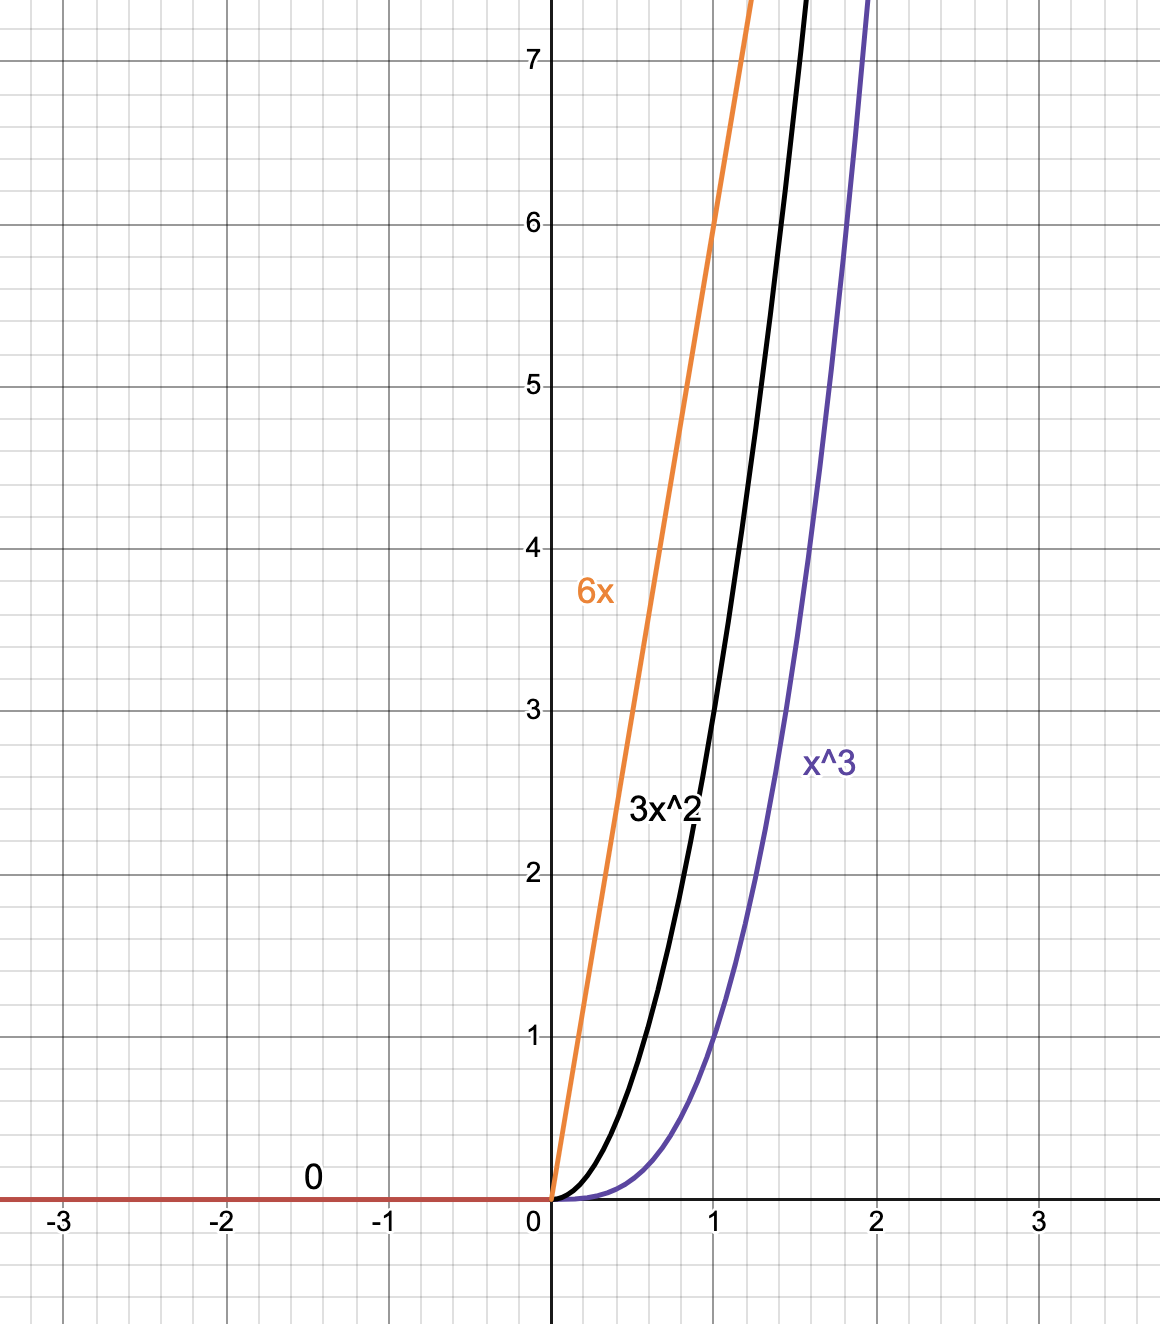
\includegraphics[width=0.5\linewidth]{Math 134/Images/ggraph.png}
\end{figure}
    \end{enumerate}

    \item [\textbf{61. }]To prove: If \( y = x^{-1} \), then the \( n \)-th derivative of \( y \) is \( \frac{d^ny}{dx^n} = (-1)^n \cdot n! \cdot x^{-n-1} \).
    \begin{enumerate}

    For \( n = 0 \), the \( 0 \)-th derivative is simply \( y(x) \), so
    \[
    y = x^{-1}
    \]
    which matches the formula for \( n = 0 \):
    \[
    (-1)^0 \cdot 0! \cdot x^{-0-1} = 1 \cdot 1 \cdot x^{-1} = x^{-1}
    \]
    Thus, the base case holds.

    Assume that for some \( n = k \), the formula holds,
    \[
    \frac{d^ky}{dx^k} = (-1)^k \cdot k! \cdot x^{-k-1}
    \]

 Inductive Step: Differentiate \( \frac{d^ky}{dx^k} = (-1)^k \cdot k! \cdot x^{-k-1} \) using the power rule:
    \[
    \frac{d^{k+1}y}{dx^{k+1}} = \frac{d}{dx}\left(\frac{d^{k}y}{dx^{k}}\right)
    \]
    \[
    \frac{d^{k+1}y}{dx^{k+1}}= \frac{d}{dx} \left( (-1)^k \cdot k! \cdot x^{-k-1} \right) = (-1)^k \cdot k! \cdot (-k-1) \cdot x^{-k-2}
    \]
    Simplifying:
    \[
    \frac{d^{k+1}y}{dx^{k+1}}= (-1)^k \cdot k! \cdot -1\cdot(k+1) \cdot x^{-k-2} = (-1)^{k+1} \cdot (k+1)! \cdot x^{-k-2}
    \]
    The result obtained by differentiating the $k^{th}$ derivative of $y$ results in the $k+1^{th}$ derivative of $y$ according to the proposed formula. Thus, we can say the formula holds true for all $n\in \mathbb{N}$.
    \end{enumerate}

    \item [\textbf{62. }]
    \begin{enumerate}
    \item If \( f(x) \) is even, then \( f'(x) \) is odd.

    A function \( f(x) \) is even if \( f(-x) = f(x) \) for all \( x \).

    We are given that \( f(x) \) is even, so \( f(-x) = f(x) \). Differentiating both sides:
    \[
    \frac{d}{dx} f(-x) = \frac{d}{dx} f(x)
    \]
    By the chain rule, the derivative of \( f(-x) \) is:
    \[
    \frac{d}{dx} f(-x) = f'(-x) \cdot \frac{d}{dx}(-x) = f'(-x) \cdot (-1) = -f'(-x)
    \]
    The derivative of \( f(x) \) on the right-hand side is just \( f'(x) \), so:
    \[
    -f'(-x) = f'(x)
    \]
    Rearranging the equation gives:
    \[
    f'(-x) = -f'(x)
    \]
    The above is the definition of an odd function. Thus if $f(x)$ is even, then $f'(x)$ is odd
    \bigbreak

    \item If \( f(x) \) is odd, then \( f'(x) \) is even.

    A function \( f(x) \) is odd if \( f(-x) = -f(x) \) for all \( x \).

    We are given that \( f(x) \) is odd, so \( f(-x) = -f(x) \). Differentiating both sides:
    \[
    \frac{d}{dx} f(-x) = \frac{d}{dx} [-f(x)]
    \]
    Applying the chain rule to the left-hand side gives:
    \[
    \frac{d}{dx} f(-x) = f'(-x) \cdot \frac{d}{dx}(-x) = -f'(-x)
    \]
    The derivative of \( -f(x) \) on the right-hand side is:
    \[
    \frac{d}{dx} [-f(x)] = -f'(x)
    \]
    Equating both sides gives:
    \[
    -f'(-x) = -f'(x)
    \]
    Simplifying, we get:
    \[
    f'(-x) = f'(x)
    \]
    The above is the definition of an even function. Thus if $f(x)$ is odd, then $f'(x)$ is even
    \end{enumerate}
\newpage
    \item [\textbf{67.}] 
    \begin{enumerate}
        \item For $x\neq 0$
        \[
        f(x) = x \sin\left(\frac{1}{x}\right) 
        \]
        Thus, by using product rule and chain rule we obtain the following:
        \[
        f'(x) = 1\left(\sin\left(\frac{1}{x}\right)\right) + x\left(\cos\left(\frac{1}{x}\right) \times \frac{-1}{x^2}\right)
        \]
        This simplifies to:
        \[
        f'(x) =\sin\left(\frac{1}{x}\right) -\frac{\cos\left(\frac{1}{x}\right)}{x}
        \]

        \[
        g(x) = x^2\sin\left(\frac{1}{x}\right)
        \]
        Using product rule and chain rule:
        \[
        g'(x) = 2x\sin\left(\frac{1}{x}\right) + x^2\left(\cos\left(\frac{1}{x}\right) \times \frac{-1}{x^2}\right)
        \]
        Simplifying
        \[
        g'(x) = 2x\sin\left(\frac{1}{x}\right) - \cos\left(\frac{1}{x}\right)
        \]
        \item 
        If $g'(x)$ was continuous at 0:
        \[
        \lim_{x\to0} g'(x) = g(0)
        \]

        \[
        \lim_{x \to 0}2x\sin\left(\frac{1}{x}\right)- \cos\left(\frac{1}{x}\right)
        \]
        Using the limit theorem, 
        \[
        \lim_{x\to0}2x\sin\left(\frac{1}{x}\right) - \lim_{x\to0}\cos\left(\frac{1}{x}\right)
        \]
        The following limit computes to 0 as $2x$ approaches 0
        \[
        \lim_{x\to0}2x\sin\left(\frac{1}{x}\right) = 0
        \]
        However, the following limit exhibits oscillating behaviour, thus the limit does not exist at 0. Thus, $g'(x)$ is not continuous at 0.
        
    \end{enumerate}

    \item [\textbf{72.}]
    \begin{enumerate}
        \item 
        \[
        \theta(t) = A \sin(\omega t+ \phi)
        \]
        Applying chain rule
        \[
        \theta'(t) = A \cos(\omega t + \phi) \times \omega = A\omega\cos(\omega t + \phi)
        \]
        \[
        \theta''(t) = -A\omega\sin(\omega t + \phi) \times \omega = -A\omega^2\sin(\omega t + \phi)
        \]
        Separating the $\omega^2$ term,
        \[
        \theta''(t) = -\omega^2 \times A \sin(\omega t+ \phi)
        \]
        Replacing the original function in:
        \[
        \theta''(t) = -\omega^2 \theta(t)
        \]
        Thus, we can say that $\theta(t)$ satisfies the equation
        \bigbreak
        \item 
        \[
        \theta(t) = A\sin(\omega t+\phi)
        \]
        Using the formula: $\sin(a+b) = \sin(a)\cos(b) + \cos(a)\sin(b)$
        \[
        \theta(t) = A\sin(\omega t)\cos(\phi) + A\sin(\phi)\cos(\omega t)
        \]
        Let $C = A\cos(\phi)$ and $B = A\sin(\phi)$
        \[
        \theta(t) = C\sin(\omega t) + B\cos(\omega t)
        \]
        Thus, $\theta(t)$ can be expressed in the above form.
    \end{enumerate}
\bigbreak
    \item [\textbf{52.}]

    We begin with the equation of the parabola:
    \[
    x = a y^2.
    \]
    Dividing both sides by \( y^2 \) gives:
    \[
    \frac{x}{y^2} = a.
    \]

    Now, we differentiate both sides of the equation implicitly with respect to \( x \).
    \[
    \frac{d}{dx} \left( \frac{x}{y^2} \right) = \frac{d}{dx} (a).
    \]
    The derivative of the constant \( a \) on the right-hand side is zero, so:
    \[
    \frac{d}{dx} \left( \frac{x}{y^2} \right) = 0.
    \]

    Using the quotient rule for differentiation on \( \frac{x}{y^2} \), we have:
    \[
    \frac{d}{dx} \left( \frac{x}{y^2} \right) = \frac{y^2 \cdot \frac{dx}{dx} - x \cdot \frac{d}{dx} (y^2)}{(y^2)^2}.
    \]

    Since \( \frac{dx}{dx} = 1 \) and \( \frac{d}{dx}(y^2) = 2y \frac{dy}{dx} \), this becomes:
    \[
    \frac{y^2 - x \cdot 2y \frac{dy}{dx}}{y^4} = 0.
    \]

    \[
    y^2 - 2xy \frac{dy}{dx} = 0.
    \]
    Solving for \( \frac{dy}{dx} \) gives:
    \[
    2xy \frac{dy}{dx} = y^2,
    \]
    \[
    \frac{dy}{dx} = \frac{y^2}{2xy} = \frac{y}{2x}.
    \]

    Thus, the slope of the tangent to the parabola is:
    \[
    m_{\text{parabola}} = \frac{y}{2x}.
    \]



    Next, for the ellipse equation \( x^2 + \frac{y^2}{2} = b \), we differentiate both sides implicitly with respect to \( x \):
    \[
    2x + y \frac{dy}{dx} = 0.
    \]
    Solving for \( \frac{dy}{dx} \) gives:
    \[
    \frac{dy}{dx} = -\frac{2x}{y}.
    \]

    For the curves to be orthogonal at their points of intersection, the product of their slopes must equal \(-1\):
    
    \[
    -1 = -1.
    \]
    \[
    -\frac{y}{2x} \cdot \frac{2x}{y} = -1,
    \]
    \[
    m_{\text{parabola}} \cdot m_{\text{ellipse}} = -1.
    \]

    Thus, they are orthogonal\\
    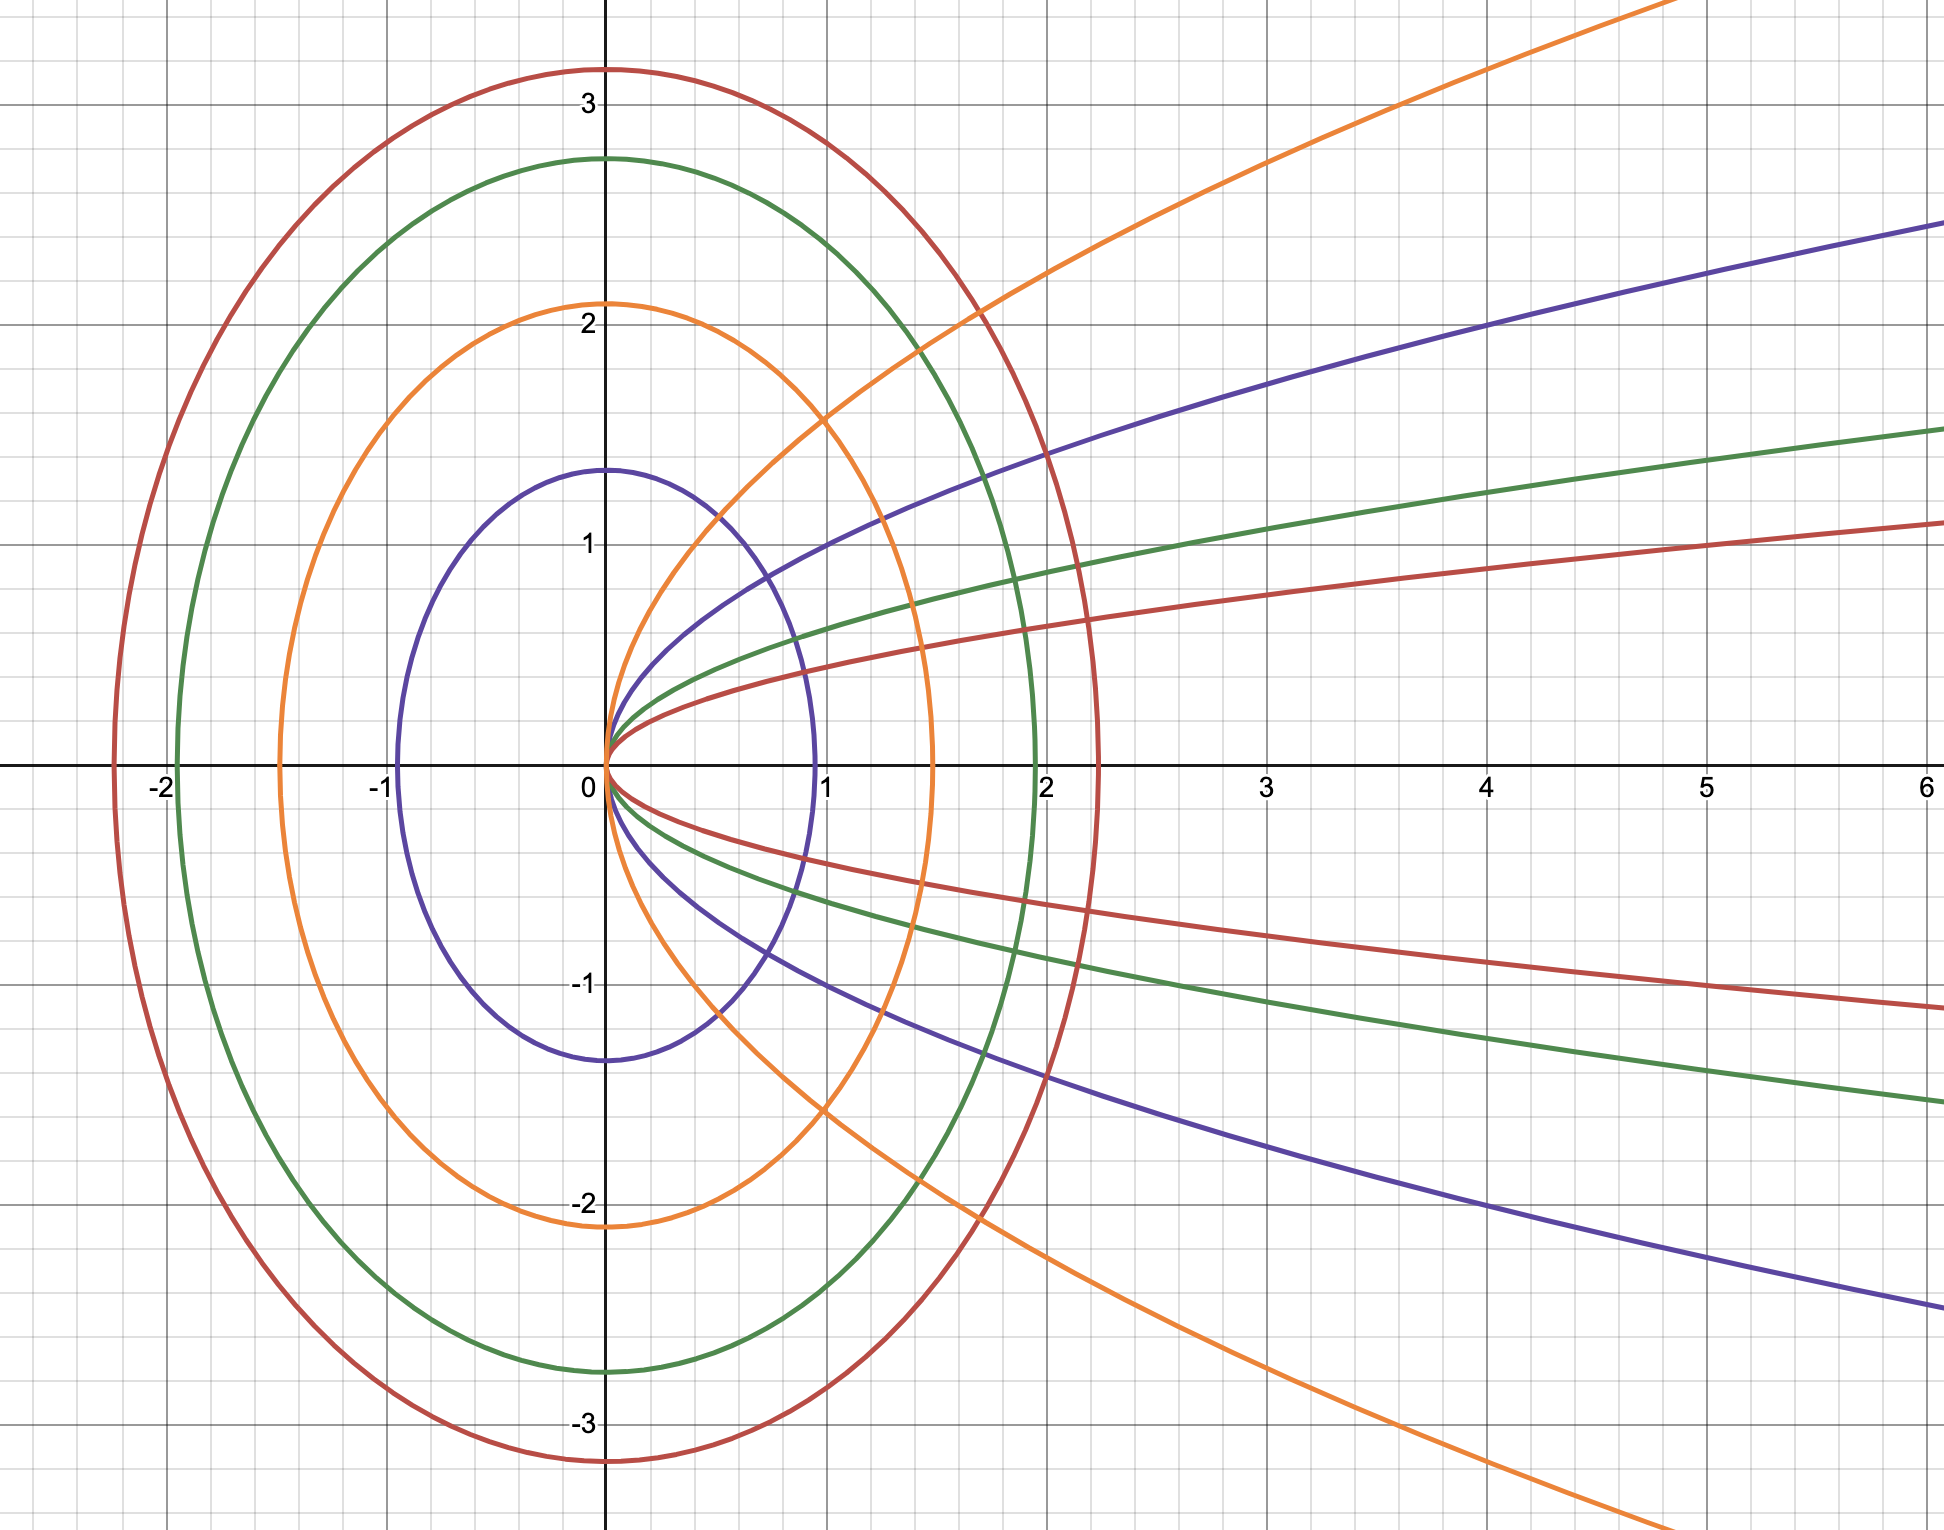
\includegraphics[width=0.5\linewidth]{Math 134/Images/ellpise.png}
    

    \item [\textbf{55.}]

    We start with the equation of the lemniscate:
    \[
    (x^2 + y^2)^2 = x^2 - y^2.
    \]

    We will differentiate both sides with respect to \( x \).

    Using the chain rule and implicit differentiation:
    \[
    \frac{d}{dx}[(x^2 + y^2)^2] = \frac{d}{dx}[x^2 - y^2].
    \]

    Using the chain rule on the left side:
    \[
    2(x^2 + y^2)(2x + 2y \frac{dy}{dx}) = 2x - 2y \frac{dy}{dx}.
    \]

    Simplifying:
    \[
    2(x^2 + y^2)(x + y \frac{dy}{dx}) = x - y \frac{dy}{dx}.
    \]

    Rearranging gives:
    \[
    2(x^2 + y^2)x + 2(x^2 + y^2)y \frac{dy}{dx} = x - 2(x^2 + y^2)x.
    \]

    Combine the terms involving \(\frac{dy}{dx}\):
    \[
    2(x^2 + y^2)y \frac{dy}{dx} + y \frac{dy}{dx} = x - 2(x^2 + y^2)x.
    \]

    Factoring out \(\frac{dy}{dx}\):
    \[
    \left(2(x^2 + y^2)y + y\right) \frac{dy}{dx} = x - 2(x^2 + y^2)x.
    \]

    Thus, we have:
    \[
    \frac{dy}{dx} = \frac{x - 2(x^2 + y^2)x}{2(x^2 + y^2)y + y}.
    \]

    Setting the numerator equal to zero gives the condition for horizontal tangents:
    \[
    x - 2(x^2 + y^2)x = 0.
    \]
    This simplifies to:
    \[
    x(1 - 2(x^2 + y^2)) = 0.
    \]

    This yields two cases:
    
    1. \(x = 0\)\\
    2. \(1 - 2(x^2 + y^2) = 0\) or \(x^2 + y^2 = \frac{1}{2}\)

    Case 1: \(x = 0\)

    Substituting \(x = 0\) into the original equation:
    \[
    (0^2 + y^2)^2 = 0^2 - y^2 \implies y^4 = -y^2.
    \]
    This gives:
    \[
    y^4 + y^2 = 0 \implies y^2(y^2 + 1) = 0.
    \]
    Thus, \(y^2 = 0\) or \(y^2 = -1\), which gives \(y = 0\).

    Thus, we have one point:
    \[
    (0, 0).
    \]

    Case 2: \(x^2 + y^2 = \frac{1}{2}\)

    Substituting this back into the lemniscate equation:
    \[
    \left(\frac{1}{2}\right)^2 = x^2 - y^2 \implies \frac{1}{4} = x^2 - y^2.
    \]
    Now, substituting \(y^2 = \frac{1}{2} - x^2\):
    \[
    \frac{1}{4} = x^2 - \left(\frac{1}{2} - x^2\right).
    \]
    This simplifies to:
    \[
    \frac{1}{4} = x^2 - \frac{1}{2} + x^2,
    \]
    \[
    \frac{1}{4} = 2x^2 - \frac{1}{2}.
    \]
    Multiplying through by 4 gives:
    \[
    1 = 8x^2 - 2 \implies 8x^2 = 3 \implies x^2 = \frac{3}{8} \implies x = \pm\sqrt{\frac{3}{8}}.
    \]

    Now substituting \(x^2 = \frac{3}{8}\) back to find \(y^2\):
    \[
    y^2 = \frac{1}{2} - \frac{3}{8} = \frac{4}{8} - \frac{3}{8} = \frac{1}{8} \implies y = \pm \sqrt{\frac{1}{8}}.
    \]

    This gives us four points:
    
    1. \(\left(\sqrt{\frac{3}{8}}, \sqrt{\frac{1}{8}}\right)\)\\
    2. \(\left(\sqrt{\frac{3}{8}}, -\sqrt{\frac{1}{8}}\right)\)\\
    3. \(\left(-\sqrt{\frac{3}{8}}, \sqrt{\frac{1}{8}}\right)\)\\
    4. \(\left(-\sqrt{\frac{3}{8}}, -\sqrt{\frac{1}{8}}\right)\)\\

    Thus, the four points of the curve at which the tangent line is horizontal are:
    1. \(\left(\sqrt{\frac{3}{8}}, \sqrt{\frac{1}{8}}\right)\)\\
    2. \(\left(\sqrt{\frac{3}{8}}, -\sqrt{\frac{1}{8}}\right)\)\\
    3. \(\left(-\sqrt{\frac{3}{8}}, \sqrt{\frac{1}{8}}\right)\)\\
    4. \(\left(-\sqrt{\frac{3}{8}}, -\sqrt{\frac{1}{8}}\right)\)\\

\item [\textbf{58.}] 
    The equation of the circle with center \( (0, a) \) and radius \( 1 \) is given by:
    \[
    (x - 0)^2 + (y - a)^2 = 1.
    \]
    Simplifying this gives:
    \[
    x^2 + (y - a)^2 = 1.
    \]
    The parabola is given by \( y = 2x^2 \).

    We substitute the parabola equation into the circle's equation:
    \[
    x^2 + (2x^2 - a)^2 = 1.
    \]

    So, the equation becomes:
    \[
    x^2 + 4x^4 - 4ax^2 + a^2 = 1.
    \]
    Rearranging gives:
    \[
    4x^4 + (1 - 4a)x^2 + (a^2 - 1) = 0.
    \]

    This is a quadratic equation in \( x^2 \). For the circle to be inscribed, this equation must have a double root. Therefore, the discriminant must be zero.

    The discriminant \( D \) of the quadratic \( Ax^2 + Bx + C = 0 \) is given by \( D = B^2 - 4AC \). Here:
    \[
    A = 4, \quad B = 1 - 4a, \quad C = a^2 - 1.
    \]
    Thus, the discriminant becomes:
    \[
    D = (1 - 4a)^2 - 4(4)(a^2 - 1) = 0.
    \]

    Setting the discriminant equal to zero:
    \[
    (1 - 4a)^2 - 16(a^2 - 1) = 0.
    \]

    Expanding this gives:
    \[
    1 - 8a + 16a^2 - 16a^2 + 16 = 0.
    \]
    Simplifying, we have:
    \[
    -8a + 17 = 0.
    \]
    Solving for \( a \):
    \[
    8a = 17 \quad \Rightarrow \quad a = \frac{17}{8}.
    \]

    Now we substitute \( a \) back into the quadratic equation to find \( x^2 \):
    \[
    4x^4 + (1 - 4 \cdot \frac{17}{8})x^2 + \left(\left(\frac{17}{8}\right)^2 - 1\right) = 0.
    \]

    So the equation becomes:
    \[
    4x^4 - \frac{15}{2}x^2 + \left(\frac{289}{64} - 1\right) = 0.
    \]

    Now our equation simplifies to:
    \[
    4x^4 - \frac{15}{2}x^2 + \frac{225}{64} = 0.
    \]
    Multiplying through by \( 64 \) to eliminate fractions:
    \[
    256x^4 - 480x^2 + 225 = 0.
    \]

 
    Using the quadratic formula:
    \[
    x = \frac{-(-480) \pm \sqrt{(-480)^2 - 4 \cdot 256 \cdot 225}}{2 \cdot 256}.
    \]
    Calculating the discriminant:
    \[
    (-480)^2 = 230400,
    \]
    \[
    4 \cdot 256 \cdot 225 = 230400.
    \]
    Thus, the discriminant is:
    \[
    D = 230400 - 230400 = 0.
    \]
    Since the discriminant is zero, there is one double root:
    \[
    x^2 = \frac{480}{2 \cdot 256} = \frac{480}{512} = \frac{15}{16}.
    \]
    \[
    x = \pm \frac{\sqrt{15}}{4}.
    \]

    Using \( y = 2x^2 \):
    \[
    y = 2 \cdot \frac{15}{16} = \frac{30}{16} = \frac{15}{8}.
    \]

    The points of contact are:
    \[
    \left(\frac{\sqrt{15}}{4}, \frac{15}{8}\right) \quad \text{and} \quad \left(-\frac{\sqrt{15}}{4}, \frac{15}{8}\right).
    \]
\end{enumerate}
\end{document}
